\documentclass[12pt]{article}
\usepackage[letterpaper]{geometry}
\usepackage{graphicx}
\usepackage{flafter}
\usepackage{enumitem}
\usepackage{float}
\usepackage{longtable}
\usepackage{tabularx}
\usepackage{multicol}
\usepackage{amsmath,amsthm,amssymb, amsthm}
\usepackage{enumitem}
\usepackage{mathtools}
\usepackage{listings}
\usepackage{mathptmx}
\setlist[itemize]{itemsep=0mm}
\usepackage[font=small,labelfont=bf]{caption}
\usepackage[capitalise]{cleveref}
\usepackage{setspace}
\usepackage{afterpage}
\usepackage[authoryear,round,longnamesfirst]{natbib}
\usepackage{bibentry}

\newcounter{protocol}
\newenvironment{protocol}[1]
  {\par\addvspace{\topsep}
   \noindent
   \tabularx{\linewidth}{@{} X @{}}
    \hline
    \refstepcounter{protocol}\textbf{Protocol \theprotocol} #1 \\
    \hline}
  { \\
    \hline
   \endtabularx
   \par\addvspace{\topsep}}

 \newcommand{\sbline}{\\[.5\normalbaselineskip]}% small blank line

\newcommand{\set}[1]{\left\{#1\right\}}
\newcommand{\setc}[2]{\left\{#1 \; :\; #2 \right\}}

% \doublespacing


\title{Implementing Stateless Clients in Ethereum}
\author{Souvik Banerjee}
\date{}

\begin{document}
\maketitle

\section{Abstract}

\section{Introduction}

% reword first two sentences

In the last few years, blockchain technology has become increasingly popular.
Blockchain is a decentralized data sharing technology that works in a distributed environment consisting of multiple nodes. It can be defined as a immutable \emph{ledger} that records transactions. The blockchain structure consists of cryptographically signed \emph{blocks} that are linked to each other with cryptographic hashes. Each block contains \emph{transactions} that show value transfers between different accounts. Each node in the network maintains its own copy of the blockchain, which makes the ledger a \emph{distributed ledger}. The ledger is kept up to date using a distributed consensus mechanism, which allows nodes to validate transactions, package them into blocks, and update the block hash chain.

Blockchain and cryptocurrency are two different concepts, but their development has been intertwined. Blockchain was first suggested by Satoshi Nakamoto's paper introducing Bitcoin in late 2008. Bitcoin is a cryptocurrency and is a specific implementation of blockchain technology.

Ethereum is a cryptocurrency that builds upon the ideas introduced in Bitcoin. Ethereum is a transaction-based state machine that starts with some initial \emph{genesis} state, incrementally executes transactions, and arrives at a final state. These transactions are collected into blocks, and blocks are hashed to create a hash chain. The Ethereum protocol has a native currency called Ether and is abbreviated as ETH.

The goal of Ethereum is to create a platform for decentralized applications, and it does this by incorporating a built-in Turing complete programming language. This allows users to write \emph{smart contracts} that contain arbitrary code and run on the decentralized Ethereum network. In contrast to Bitcoin, where transactions are simply value transfers between accounts, Ethereum transactions can create and run smart contracts. The ability to run arbitrary code makes Ethereum an extremely powerful abstraction layer on which decentralized applications can be built.

One problem with blockchain-based systems is that they are orders of magnitude slower than their centralized equivalent. Ethereum is only able to process about 15 transactions per second, while payment processors like Visa can process 24,000 transactions per second. New distributed applications that run on Ethereum such as CryptoKitties have slowed down transaction processing time even further. Improving scalability of blockchain-based systems is crucial for widespread adoption.

A proposed solution to Ethereum's scalability problems is called \emph{stateless clients}. Stateless Clients was proposed by Vitalik Buterin, the founder of Ethereum, in 2017. Stateless Clients aims to improve scalability by reducing I/O when verifying blocks. However, until now there has been no working prototype of stateless clients.

The structure of this paper is as follows: first, I will review some foundational concepts in Ethereum. Second, I will describe in more detail how Stateless Clients is designed and how I implemented Stateless Clients in Parity. Third, I will show some of the results I obtained from my implementation.

\section{Background}

\subsection{Ethereum Virtual Machine}

Ethereum is a platform for deploying and running smart contracts. Smart contracts are programs that enforce a contract and run in the Ethereum Virtual Machine, or EVM. Smart contracts are created with the \emph{Solidity} programming language, and compile to EVM opcodes. The Ethereum blockchain is replicated on many nodes and all nodes verify the correct execution of the smart contract. This makes smart contracts useful for self-executing agreements between two parties.

These EVM opcodes allow the EVM to be Turing complete, limited only by the following factors:
\begin{enumerate}
  \item Stack space: The stack has a capacity of 1024 entries, and each entry is 256 bits. The EVM is a stack-based virtual machine and the stack is used to push arguments to opcodes.
  \item Execution time: Ethereum measures ``computational effort'' using \emph{gas}. Each opcode in a contract requires a certain amount of gas to pay for its execution. Contracts run as part of transactions, and one field in the transaction is called the \emph{gas price}. In order to pay for a contract's execution, the amount of gas consumed during the execution is multiplied by the gas price, and resulting product is deducted from the transaction sender's account.
  \item Memory: Memory is used for storing variables and calling functions. No hard limit exists on the amount of memory that may be used, but memory must be paid for with gas. The cost grows quadratically according to the following equation.
  % Equation 296 in the Yellow Paper
  \begin{align*}
    C_{mem}(a) &\equiv G_{memory} \cdot a + \lfloor \frac{a^2}{512} \rfloor \\
  \end{align*}
  $G_{memory}$ is a constant defined to be $G_{memory} = 3$, and $a$ is the amount of $256$-bit words used.
  \item Storage: Contracts may also store and read data in permanent storage. The \texttt{SSTORE} opcode stores a value to contract storage. This opcode costs 5,000 gas when writing to an existing value and 20,000 gas when writing to a new value. There is no hard limit on contract storage, but it is stored on each Ethereum node and is limited by hard drive capacity. Therefore, to discourage overuse of contract storage, the gas price is very high.
\end{enumerate}



\subsection{Ethereum Transactions and Blocks}

\emph{Transactions} are how the outside world communicates with Ethereum. A transaction can either transfer ETH between two accounts, create a smart contract, or call a smart contract. A transaction has a \emph{sender} and a \emph{receiver} which are identified by account addresses.

Each account in Ethereum is identified by a 160-bit address, and accounts can either belong to smart contracts or individuals. Smart contract addresses are determined when a contract is created using metadata from the account of the contract creator (the sender of the contract create transaction). Individual accounts use public and private keys, and the account address is the rightmost 160 bits of the SHA-3 (Keccak) hash of the public key. % footnote: explain Keccak vs SHA-3???

\begin{figure}[H]
  \centering
  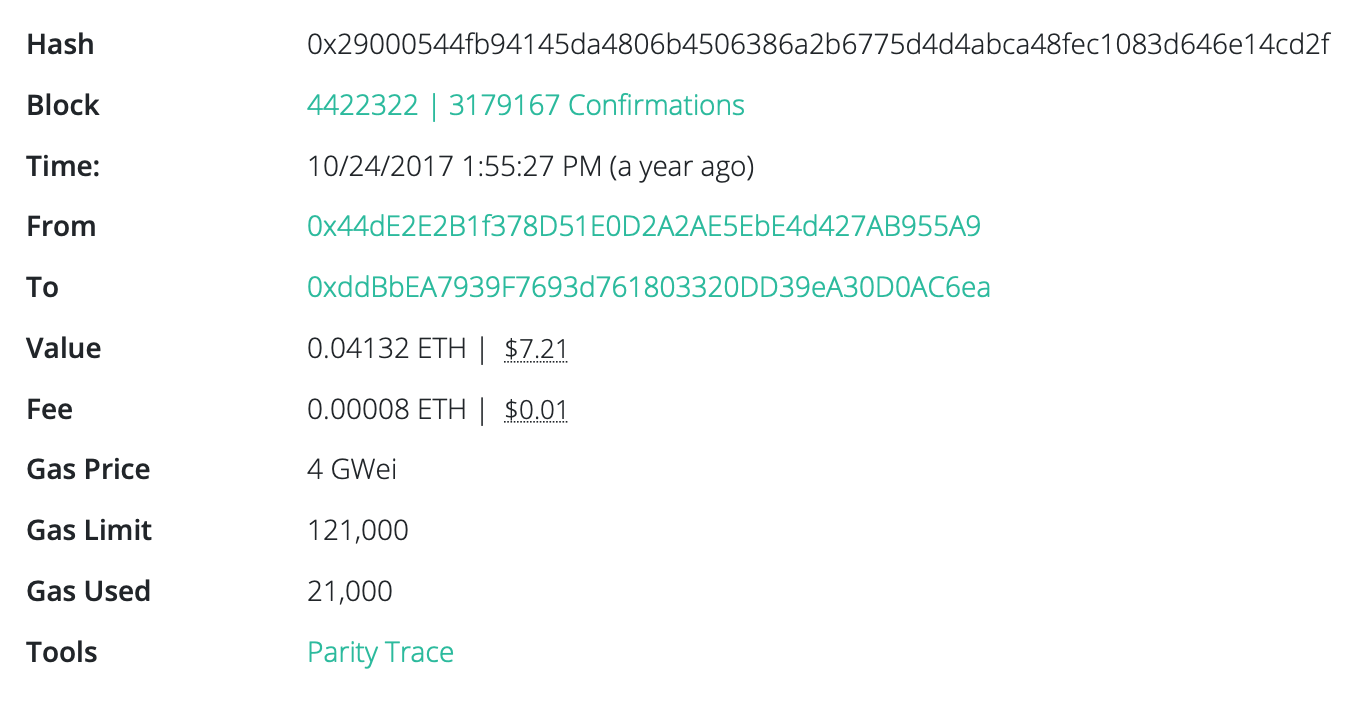
\includegraphics[width=\textwidth]{../figures/background/transactions/example_transaction.png}
  \caption{An example transaction, with sender and receiver addresses. Transactions are uniquely identified by their hash.}
\end{figure}

\emph{Blocks} in Ethereum are collections of transactions. Blocks contain transactions and a \emph{header}, which contains metadata about the block. One field in the header is the \emph{parent block hash}. Blocks ``build'' on top of previous blocks by including the SHA-3 hash of the previous block in the block header. This forms a ``hash chain'' of blocks. The hash chain makes it impossible to modify previous blocks, since doing so would change the hash of the modified block and all blocks afterwards.

\begin{figure}[H]
  \centering
  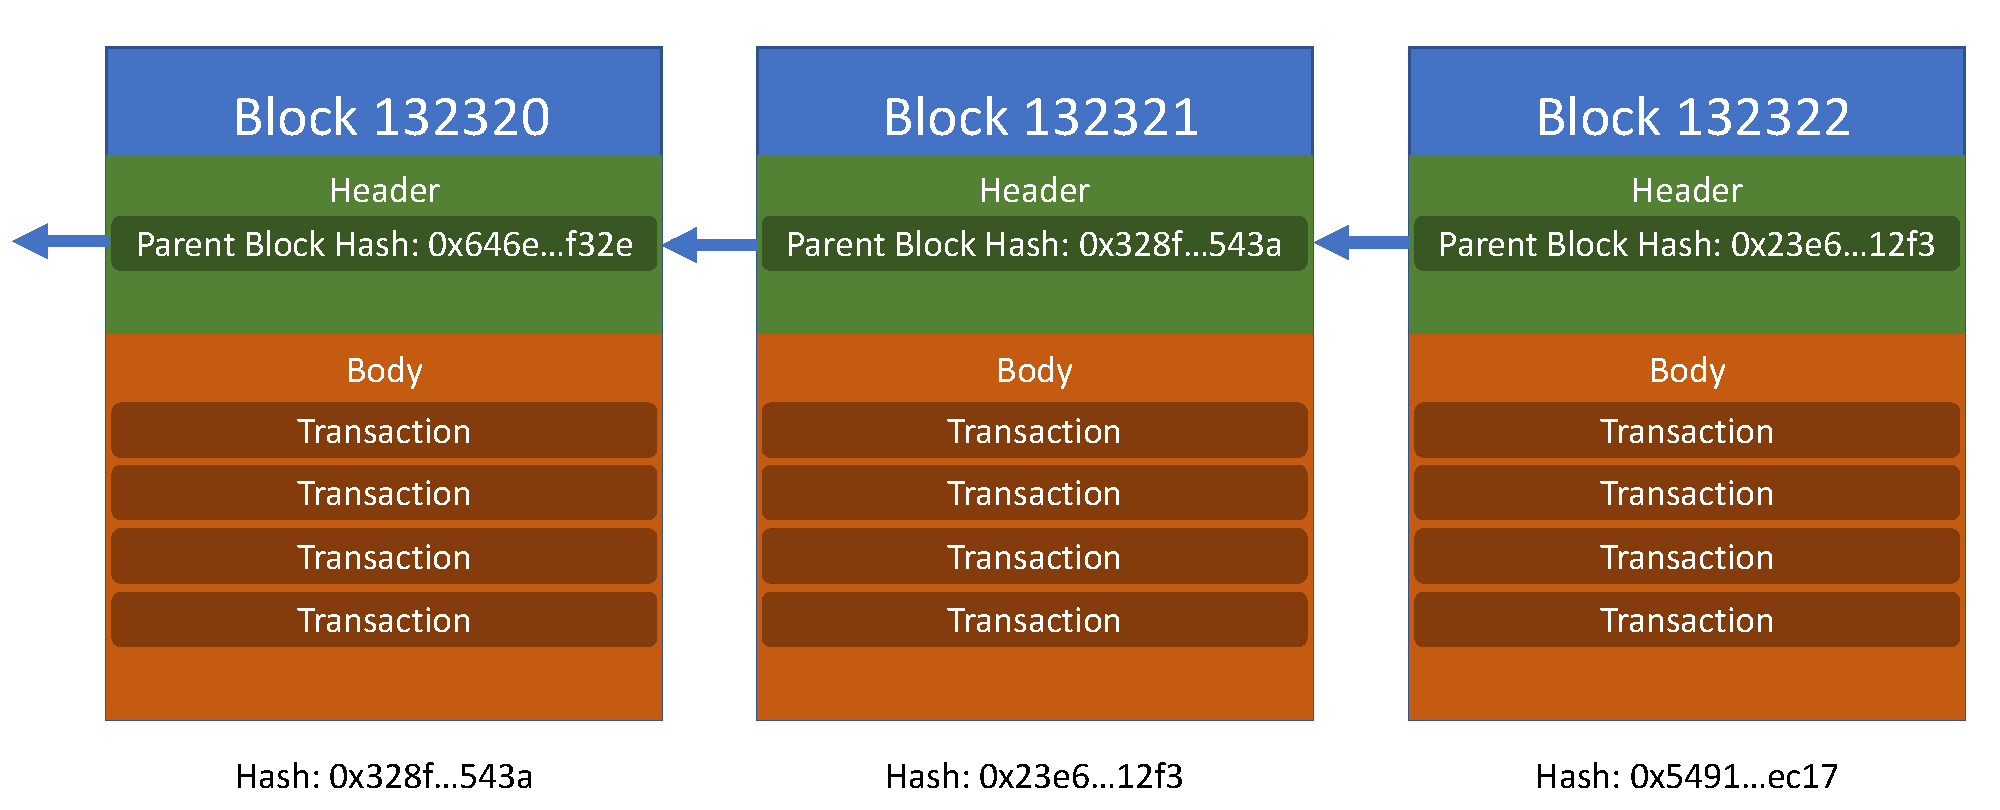
\includegraphics[width=\textwidth]{../figures/background/blocks/blocks.pdf}
  \caption{A block hash chain with 132322 blocks; the last 3 blocks are displayed. Block hashes are shown below each block. The full hash is 256 bits, but only the first and last 16 bits are shown for gbrevity.}
\end{figure}


\subsection{Recursive-Length-Prefix (RLP) Encoding}

Ethereum has a native serialization encoding called Recursive Length Prefix (RLP). RLP encodes arbitrarily nested lists of binary data. It is similar to other encoding schemes like JSON, but the range of types that are supported are limited to only lists and binary data. RLP is used to serialize blocks, transactions, and other data structures used in Ethereum.

\subsection{Merkle-Patricia Trie}

Ethereum stores account balances and other account metadata in a data structure called a \emph{Merkle-Patricia trie}. A Merkle-Patricia trie builds upon both radix tries and Merkle trees. Each node in the trie is hashed by first serializing with RLP, then using the SHA-3 hash function. This builds a key-value map of node hashes to nodes.

\begin{figure}[H]
  \centering
  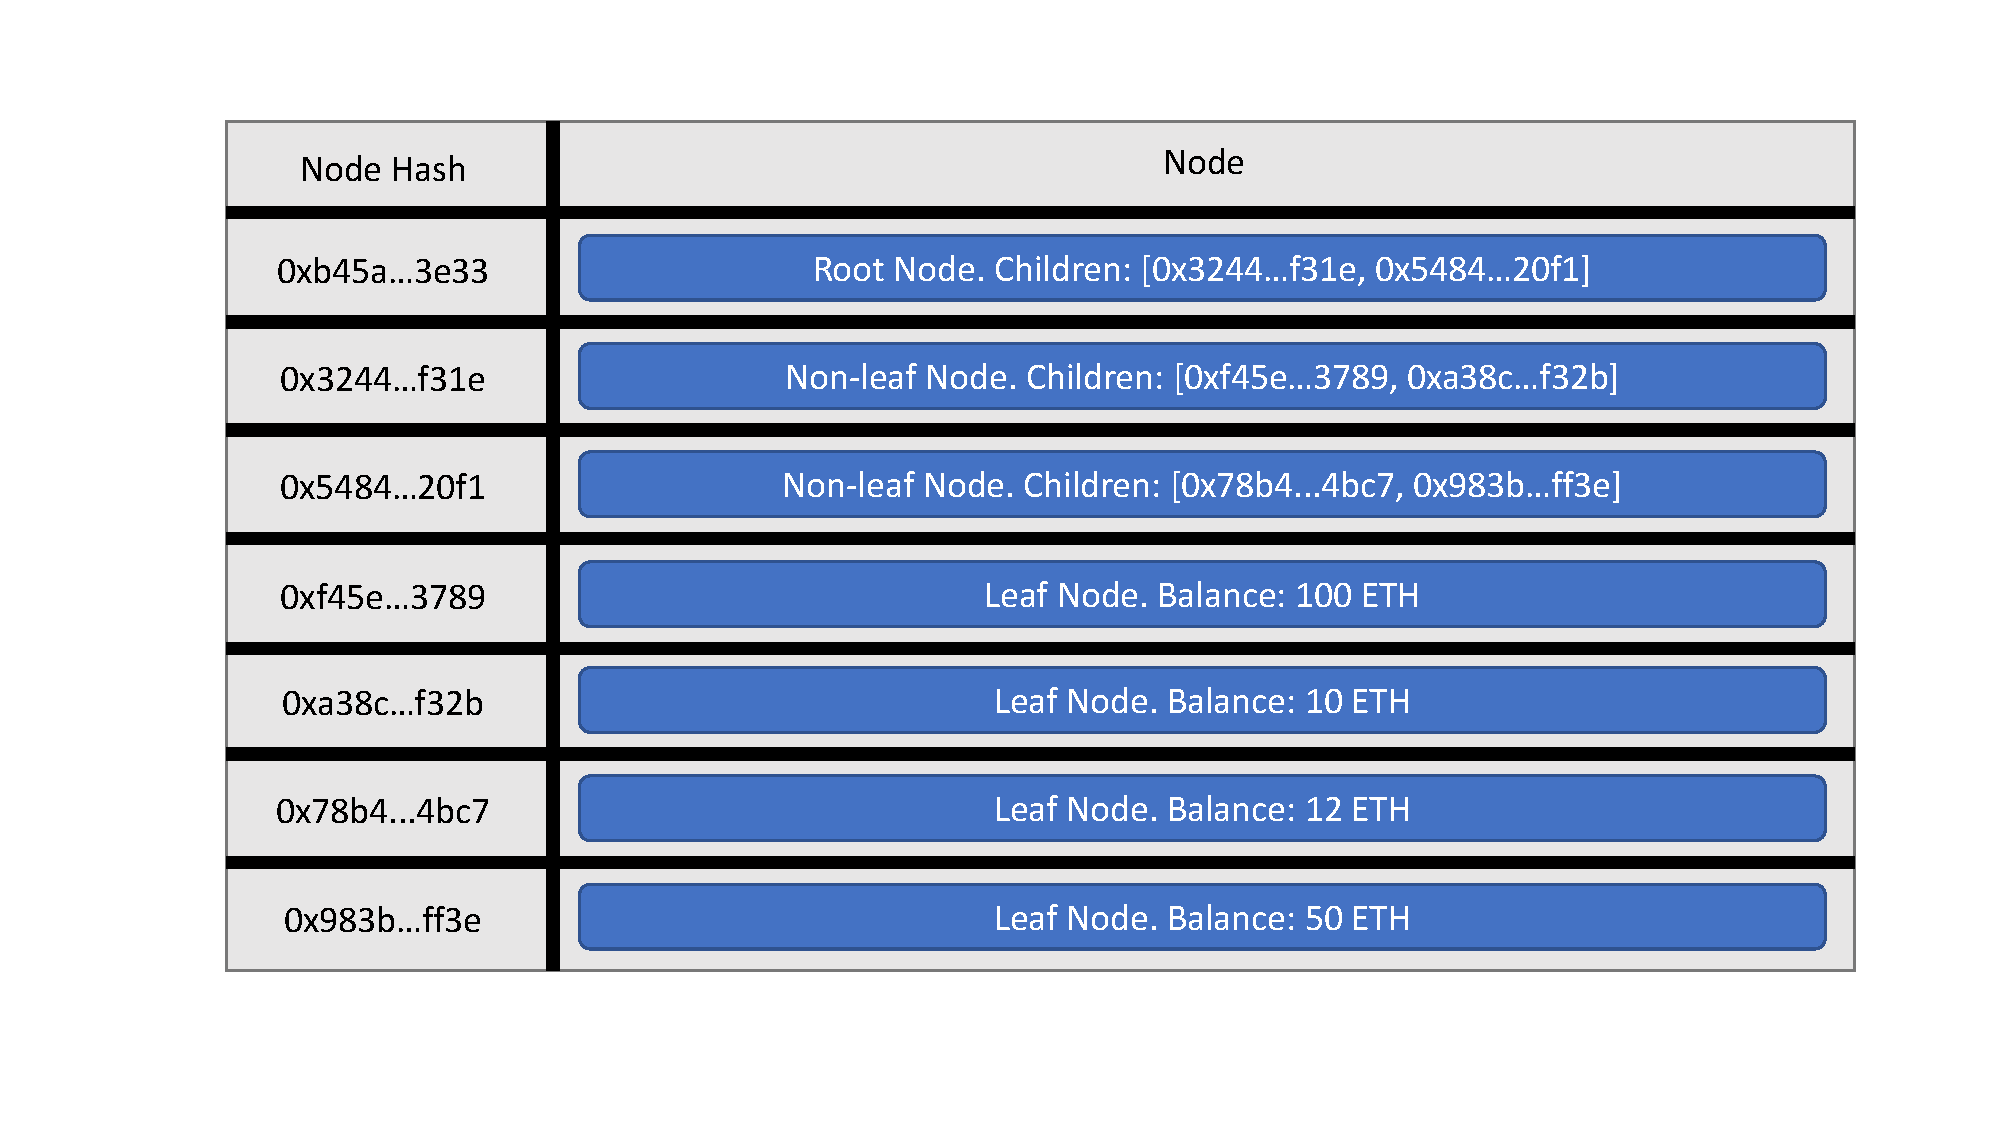
\includegraphics[width=\textwidth]{../figures/background/trie/tree_nodes.pdf}
  \caption{Trie nodes, indexed by their hash.} \label{fig:trienodes}
\end{figure}

Nodes connect with their children by using their hash, which is stored inside the node. This makes the hash of a node dependent on the hashes of its children, which are dependent on the hashes of the grandchildren, and so on. The hash of the root node can then be used to uniquely identify the entire trie.

\begin{figure}[H]
  \centering
  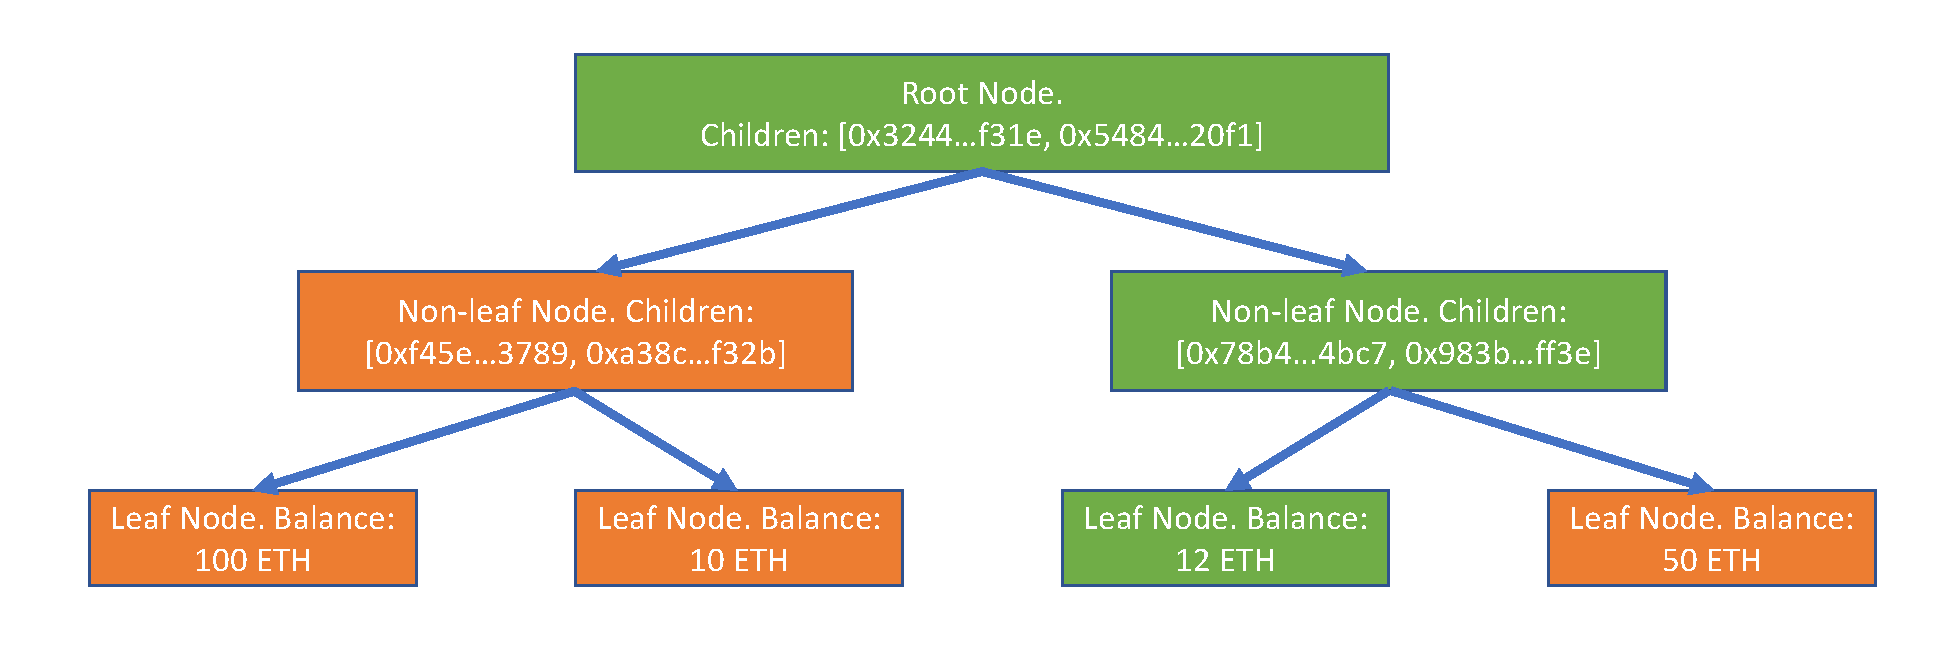
\includegraphics[width=\textwidth]{../figures/background/trie/tree_with_merkle_proof.pdf}
  \caption{The Merkle-Patricia trie. The nodes in green represent the Merkle proof for the account with a balance of 12 ETH.} \label{fig:trie}
\end{figure}

Merkle-Patricia tries also allow one to \emph{verify} values in the trie using a \emph{Merkle proof}. A Merkle proof of a value is the set of nodes along the path to the value in the trie. If someone knows the root hash of the trie, and has a Merkle proof of a value, they can verify that this value exists in the trie.


Merkle-Patricia tries are used to store the Ethereum \emph{world state}, as well as contract storage, transactions within a block, and block receipts. The Ethereum world state is the state of all accounts in Ethereum and is uniquely identified by the SHA-3 hash of the root node. Every time a value of an account changes, the hash of the root node also changes. For example, in Figure~\ref{fig:trie}, the state root hash is \texttt{0xb45a...3e33}, as shown in Figure~\ref{fig:trienodes}.

Ethereum is a transaction-based state machine, since applying a transaction to a state $S$ produces a new state $S'$. The hash of the root node (also known as the ``state root hash'') is stored in the block header, uniquely identifying the state produced after executing the transactions in that block.

 % TODO: should I go into more detail? it is pretty complicated and would take a few paragraphs to describe fully

\subsection{Consensus}
Ethereum supports multiple consensus protocols, but the protocol that is most popular is \emph{Proof-Of-Work} (PoW). Proof-of-work deters abuse by requiring that nodes perform some work. This consensus protocol requires that nodes send proofs that the work has been done. These proofs are easy to verify, but are difficult to obtain.

In the context of Ethereum, PoW is used when creating new blocks. Blocks in Ethereum must be \emph{mined} before they can be added to the hash chain. The process of mining a block is finding a
In PoW, blocks must be \emph{mined} before they are added to the hash chain. Nodes which mine blocks are called \emph{miners}. Any node in Ethereum may choose to be a miner.

Miners mine blocks by choosing values for the \emph{nonce}, a field in a block's header. A block is successfully mined if the block's hash satisfies a certain condition. By modifying the nonce field in the block header, serializing the block header with RLP, and finding the SHA-3 hash of the serialized header, we obtain the block hash. Once a nonce that satisfies the PoW condition has been found, the miner advertises the mined block on the network. Other nodes on the network check that the block has been mined correctly by hashing the block header and checking if it satisfies the PoW condition.

Miners in Ethereum are rewarded by a predetermined block reward and by the transaction fees from the transactions they include in the block. Reward distribution is done by including the account address of the miner in the block's header. This is called the block's \emph{coinbase}. Miners also do not coordinate mining blocks and race against each other to mine the next block in the block chain. Since there is no coordination, it is possible for more than one block to be generated simultaneously. If this happens, then one block will be chosen to be added onto the main block chain, and the other blocks become \emph{uncle blocks}. Miners are still rewarded for producing uncle blocks, but the reward is not as high as for producing a normal block.

% sources:
% https://www.investinblockchain.com/vitalik-ethereum-needs-100k-transactions-per-second/
% https://www.bbc.com/news/technology-42237162

\section{Design}

The stateless clients proposal, as the name suggests, changes Ethereum such that Ethereum nodes no longer need to store the Merkle-Patricia trie storing the Ethereum state. The term ``client'' is a synonym for ``node''. The proposal accomplishes this by changing the Ethereum state transition function. The original Ethereum state transition function is the following:
\begin{align*}
  STF(S, B) &\to S'
\end{align*}
Here, $S$ is the initial state, $B$ is an Ethereum block, and $S'$ is the new updated state created from applying the transactions in $B$ to $S$.

The stateless clients proposal changes the state transition function to $STF'$, which is defined here:
\begin{align*}
  STF'(r_S, B, W) \to r_{S'}
\end{align*}
Here, $r_S$ is the state root hash for $S$, $B$ is a block, and $r_{S'}$ is the state root hash for $S'$. $W$ is a ``witness'', which are Merkle proofs for each value in the state trie the execution of $B$ needs to access. These witnesses are packaged along with blocks and are sent over the network to other Ethereum nodes. Since witnesses contain the state values the execution of $B$ requires, Ethereum nodes do not need to access the state trie when verifying blocks.

The only nodes that need to access the state trie are miners. In vanilla Ethereum, miners create blocks by including transactions and performing the Proof-of-Work algorithm. The stateless clients proposal adds an additional step: generate the witness for the block. Miners need to execute the transactions in the block using their local copy of the Ethereum state trie, and keep track of which state values were accessed to obtain Merkle proofs. The set of Merkle proofs is the witness.

\subsection{Example}



\section{Implementation}

I implemented stateless clients in Parity, a popular Ethereum client written in the Rust programming language. The implementation was divided into several logical parts.

\subsection{State backend}


Ethereum state in Parity is accessed though a \texttt{State} struct. \texttt{State} handles the following tasks:
\begin{enumerate}
  \item Create recoverable checkpoints
  \item Create and retrieve smart contracts
  \item Create and retrieve account data
  \item Transfer balances between accounts
\end{enumerate}

In addition to these tasks, \texttt{State} also maintains an internal cache of the accounts that were requested. Modifications to these accounts are cached, and are written to the underlying storage only when the \texttt{State} object is destroyed.

The \texttt{State} struct provides a convenient wrapper around the Ethereum state trie. Other parts of Parity, such as the Ethereum Virtual Machine, use the functions exposed by \texttt{State} to execute transactions. However, the Ethereum state data is not stored inside the \texttt{State} object. \texttt{State} is a generic struct that uses a state backend (a \texttt{Backend} object) to read and write state data.

\texttt{Backend} is a Rust trait. Traits in Rust are similar to interfaces in other languages like Java. Structs that implement the \texttt{Backend} trait need to have the methods defined in Figure~\ref{fig:backendmethods}.

\begin{figure}[H]
  \centering
  \begin{enumerate}
    \item \texttt{Get(key)}
    \item \texttt{Insert(value)}
    \item \texttt{Emplace(key, value)}
    \item \texttt{Contains(key)}
    \item \texttt{Remove(key)}
  \end{enumerate}
  \caption{Required methods for \texttt{Backend}}
  \label{fig:backendmethods}
\end{figure}


The ``standard'' backend that Parity uses is the \texttt{StateDB} backend. \texttt{StateDB} is a struct that contains a pointer to a RocksDB database object and implements each of the required methods by reading and writing from RocksDB. RocksDB is a popular key-value store that Parity uses to store the state trie. The key for each value in the state database is simply the SHA-3 hash of the value.

\begin{figure}[H]
  \centering
  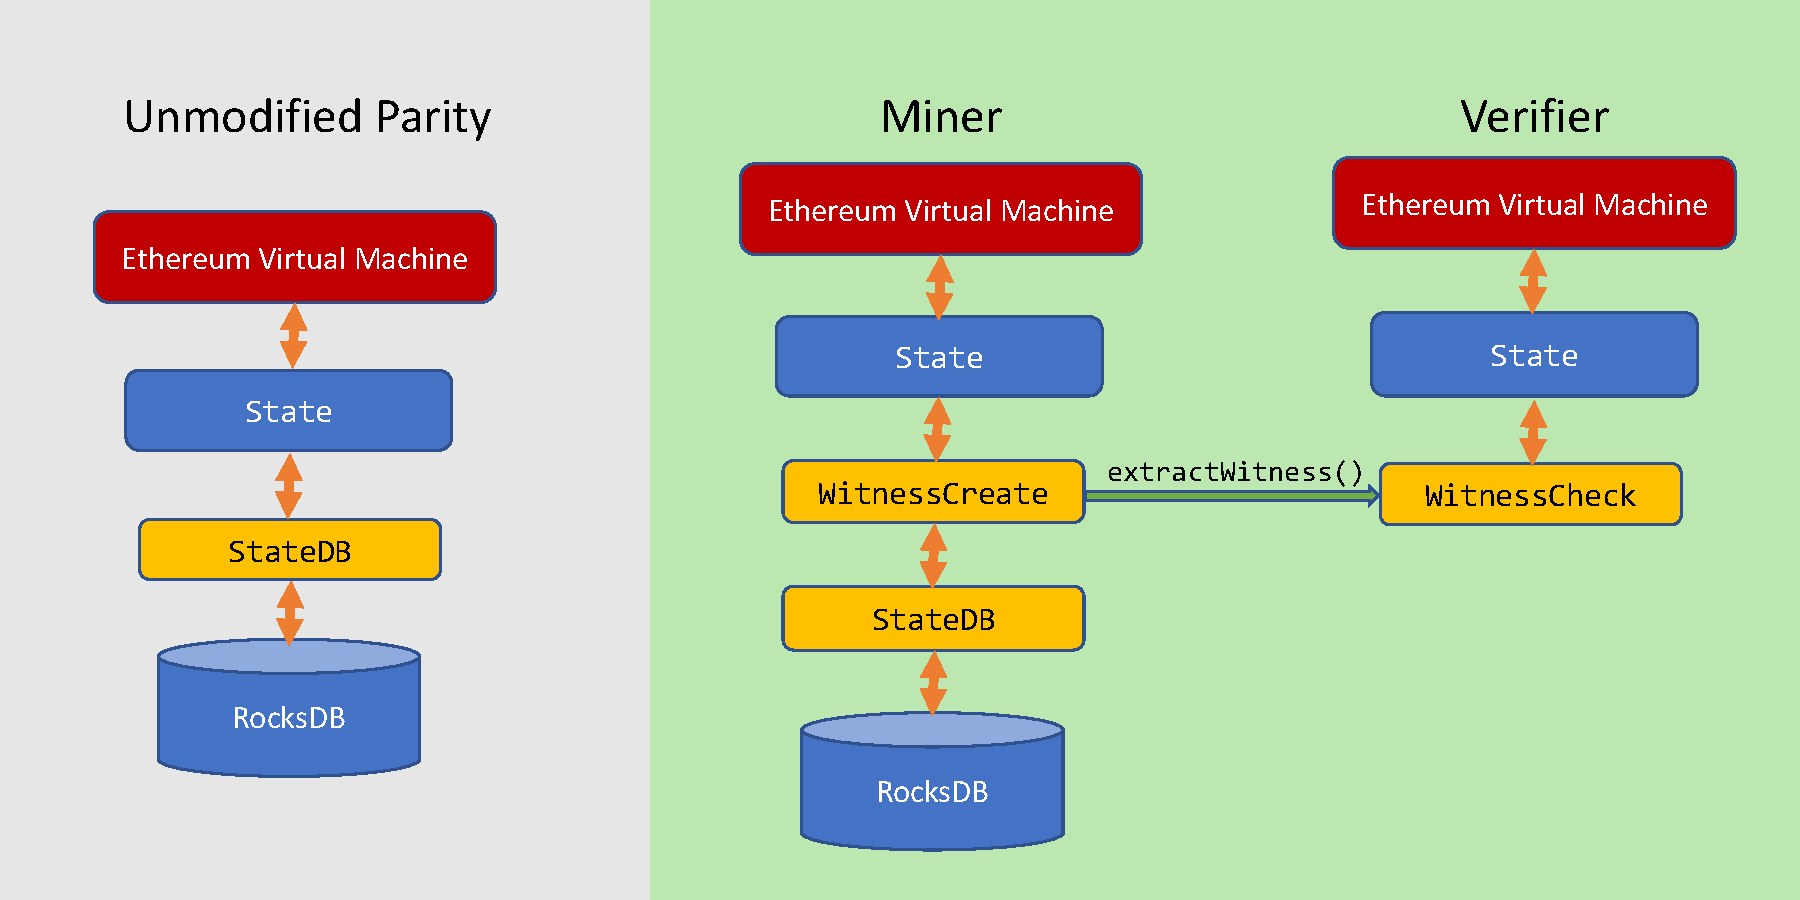
\includegraphics[width=\textwidth]{../figures/implementation/code_layout.pdf}
  \caption{The relationships between structs in Parity. In unmodified Parity, \texttt{State} communicates with \texttt{StateDB} which uses an on-disk RocksDB key-value store. In the stateless clients implementation, miners have a different code path than verifiers. Miners use \texttt{WitnessCreate} to generate witnesses by intercepting \texttt{Get()} calls to \texttt{StateDB}. Witnesses are extracted from \texttt{WitnessCreate} with \texttt{extractWitnesses()}. Verifiers use \texttt{WitnessCheck} to check these witnesses and use them as a state store for executing transactions.}
  \label{fig:parityrelationships}
\end{figure}

\subsubsection{Witness Creation}

Witnesses are generated when a block is created, and the process of block creation involves the following steps:
\begin{enumerate}
  \item Select transactions from transaction pool
  \item Execute transactions to find new state root hash
  \item Find nonce for block (``mining'')
\end{enumerate}
In Parity, blocks are created by a \texttt{Miner} object. Since the \texttt{Miner} object executes transactions, it needs access to the Ethereum state, provided by a \texttt{State} object and a \texttt{Backend} object. I replaced the \texttt{StateDB} backend that the \texttt{Miner} uses with a backend I created called \texttt{WitnessCreate}. The \texttt{WitnessCreate} backend \emph{intercepts} \texttt{Get(key)} and \texttt{Contains(key)} calls and records the values retrieved from the state database. The rest of the methods required for the \texttt{Backend} trait are implemented the same as in \texttt{StateDB}. After all transactions have been executed, the values recorded by \texttt{WitnessCreate} are extracted with a function called \texttt{extractWitness}. This witness is broadcast to the Ethereum network along with the block data once the miner successfully mines the block.

\subsubsection{Witness Verification}

Block verification in Ethereum is fairly simple. Blocks that are freshly mined are broadcast on the Ethereum network to other nodes, which download these blocks, verifies them, and finally imports them into their local block chain. Block verification has several phases:
\begin{enumerate}
  \item \texttt{verify\_block\_basic}: Checks block integrity, header parameter integrity, and verifies seals for the block and uncles
  \item \texttt{verify\_block\_unordered}: Checks transaction signatures and block nonce
  \item \texttt{verify\_block\_family}: Check block information against parent and uncle blocks.
  \item \texttt{verify\_block\_external}: Consensus engine-specific validation.
  \item \texttt{verify\_block\_final}: Executes the transactions in the block, and checks block information against block execution results. This step makes sure the resulting state root, gas used, log bloom filter, and receipts root match the what is recorded in the block header.
\end{enumerate}

I modified the final step of the block verification process to use a \texttt{WitnessCheck} state backend instead of \texttt{StateDB}. When constructing the \texttt{WitnessCheck}, we use the witness that is broadcast with the block. The \texttt{WitnessCheck} backend implements the methods in Figure~\ref{fig:backendmethods} by using the witness. \texttt{Insert(value)} and \texttt{Emplace(key, value)} are implemented by using an in-memory \texttt{HashMap} to record all write operations to the \texttt{WitnessCheck} backend. \texttt{Get(key)} is implemented by looking for values in the witness that have a SHA-3 hash equal to the \texttt{key}. If no values exist, then the in-memory \texttt{HashMap} is checked. This handles the case when a new value is written and later read from during transaction execution. \texttt{Contains(key)} is implemented by using the same logic as \texttt{Get(key)}, and \texttt{Remove(key)} only removes values from the in-memory \texttt{HashMap} leaving the witness data untouched. There are no read or write operations to the RocksDB state database when verifying blocks.

\subsection{Serialization of witnesses}
A RLP serialized block has the following layout:
\begin{enumerate}
  \item Header
  \begin{enumerate}
    \item Parent block hash
    \item Uncle block hash
    \item Block author
    \item State root hash
    \item Transaction root hash
    \item Block receipts root hash
    \item Log bloom filter
    \item Block difficulty
    \item Block number
    \item Gas limit
    \item Gas used
    \item Timestamp
    \item Extra data
  \end{enumerate}
  \item Body
  \begin{enumerate}
    \item Merkle-Patricia trie of serialized transactions
    \item Merkle-Patricia trie of headers of uncle blocks
    \item \emph{Serialized witness}
  \end{enumerate}
\end{enumerate}

I added an additional field in the \emph{Body} section of the serialized block to store the serialized block witness. The block witness is a list of database values, which can be serialized easily with RLP. The new serialized block format is used when storing blocks on disk, and when syncing blocks over the network. Adding a new field in this location maintains backwards compatibility with unmodified versions of Ethereum.

\subsection{Block sync protocol}

The block sync protocol in Ethereum also needed to be changed. Ethereum nodes use a peer-to-peer (P2P) transport protocol called RLPx to communicate between nodes. The Ethereum Wire Protocol runs on top of RLPx and is used to synchronize the following data among nodes:
\begin{enumerate}
  \item Transactions: When a node receives a transaction, it also broadcasts the same transaction to its peers.
  \item Blocks: When a node mines a new block or receives a new block from a peer, it broadcasts the same block to its peers.
  \item State: Nodes may also synchronize their state tries by broadcasting Merkle tree nodes.
\end{enumerate}


\begin{figure}[H]
  \begin{protocol}{Ethereum block synchronization protocol}
    \emph{Inputs.} Peer $P_1$ contains blocks $B_K = \set{b_{1}, b_{2}, b_{3}, \ldots, b_{K}}$, the set of blocks up to block number $K$. Peer $P_2$ contains blocks $B_H = \set{b_{1}, b_{2}, b_{3}, \ldots, b_{H}}$, the set of blocks up to block number $H$ where $H < K$.
    \sbline
    \emph{Goal.} Peer $P_2$ contains the set of blocks $B_K$.
    \sbline
    \emph{Steps:}
    \begin{enumerate}
      \item $P_1$ and $P_2$ send a \textsc{Status} message to each other.
      \item $P_2$ notices that its latest block number $H$ is less than $P_1$'s latest block number $K$. $P_2$ sends \textsc{GetBlockHeaders} to request block headers for blocks $b_{H + 1}, \ldots, b_{K}$ from $P_1$. \label{syncprotocol:requestBlockHeaders}
      \item $P_1$ replies with a \textsc{BlockHeaders} message, containing a list of block headers that $P_2$ requeested. \label{syncprotocol:replyBlockHeaders}
      \item $P_2$ sends \textsc{GetBlockBodies} to $P_1$ to request \emph{block bodies}, which are parts of the blocks excluding the header. \label{syncprotocol:requestBlockBodies}
      \item $P_1$ replies with a \textsc{BlockBodies} message, containing a list of block bodies blocks that $P_2$ requested. \label{syncprotocol:replyBlockBodies}
      \item $P_2$ matches block bodies with the block headers it received earlier using root hashes of the transaction and uncle block tries. The matched blocks form $b_{H + 1}, \ldots, b_{K}$ and are stored in $P_2$'s block chain. \label{syncprotocol:reconstruct}
    \end{enumerate}
  \end{protocol}
  \caption{Ethereum block sync protocol.} \label{syncprotocol}
\end{figure}


The block synchronization protocol flow in unmodified Ethereum is described in Figure~\ref{syncprotocol}. First, peers send a \textsc{Status} message to each other. The \textsc{Status} message notifies all participants the latest block number present in every node. Nodes that need more blocks can request blocks from the node with a greater latest block number. The key part of the sync protocol is that blocks are split in \emph{headers} and \emph{bodies} that are sent separately. First, block headers are requested and sent (step~\ref{syncprotocol:requestBlockHeaders}). Then, in step~\ref{syncprotocol:requestBlockBodies}, block bodies are requested for \emph{non-empty} blocks. Nodes are able to tell if blocks are empty by reading the block header. If a block is empty, then there is no need to request and send an empty body.


This protocol cannot be used for Stateless Clients without modifications. The reason is that no block in Stateless Clients is ``empty'', each block at least contains a witness for the block. Even if a block contains no transactions or uncle blocks, it still updates the Ethereum world state because the miner of the block gets rewarded. Rewarding the miner is done by increasing the balance in the miner's account, and the Ethereum node needs to have a Merkle proof of the balance of the miner's account.

The modifications that were made to this protocol are the following:
\begin{enumerate}
  \item In step~\ref{syncprotocol:requestBlockBodies}, peers request block bodies for \emph{all} block headers, even if the block header represents a block with no transactions or uncle blocks.
  \item In step~\ref{syncprotocol:replyBlockBodies}, peers that send block bodies also send the witness and the hash of the state root for each block body. The witness is not used in the sync protocol, but is used to reconstruct each block from its header and block body in step~\ref{syncprotocol:reconstruct}. The state root is used to match block bodies with block headers in step~\ref{syncprotocol:reconstruct}. The root hashes of the transaction trie and uncle block trie cannot be used for matching because empty blocks share the same hashes for these tries. The state root hash of a block is unique, even for empty blocks, so it may be used to match headers with block bodies.
\end{enumerate}


\section{Evaluation}

\subsection{Correctness}

I tested my implementation for stateless clients for correctness by sending blocks from one instance of Parity to another. The first instance of Parity downloaded blocks from the real Ethereum blockchain and calculated the witness for the block. It then sent the modified block to the second instance of Parity, which was running with the stateless client modifications.

The stateless client Parity instance executed each block using the provided witness for any operations involving the Ethereum state. The stateless client is only able to verify blocks with the witness correctly if the state root hash after executing the transactions within the block matches the state root hash calculated by an unmodified Parity instance. I was able to verify that all blocks in the Ethereum blockchain, up to block 7.3 million, are correctly verified by the stateless client.

\subsection{Results} \label{subsection:results}

I tested the stateless clients in a variety of experiments. The purpose of these experiments were to determine if stateless clients is a viable solution to the scalability problems in Ethereum. All experiments were run on a INSERT SYSTEM SPECIFICATIONS HERE.

\subsubsection{Witness Sizes}

The first experiment I ran measured witness sizes. I imported the first 7.3 million blocks from the Ethereum blockchain into the modified Parity Ethereum client and generated witnesses for them. The block import process is the same as the block verification process, so no changes had to be made to the client in order to generate witnesses for imported blocks.

\begin{figure}[H]
  \centering
  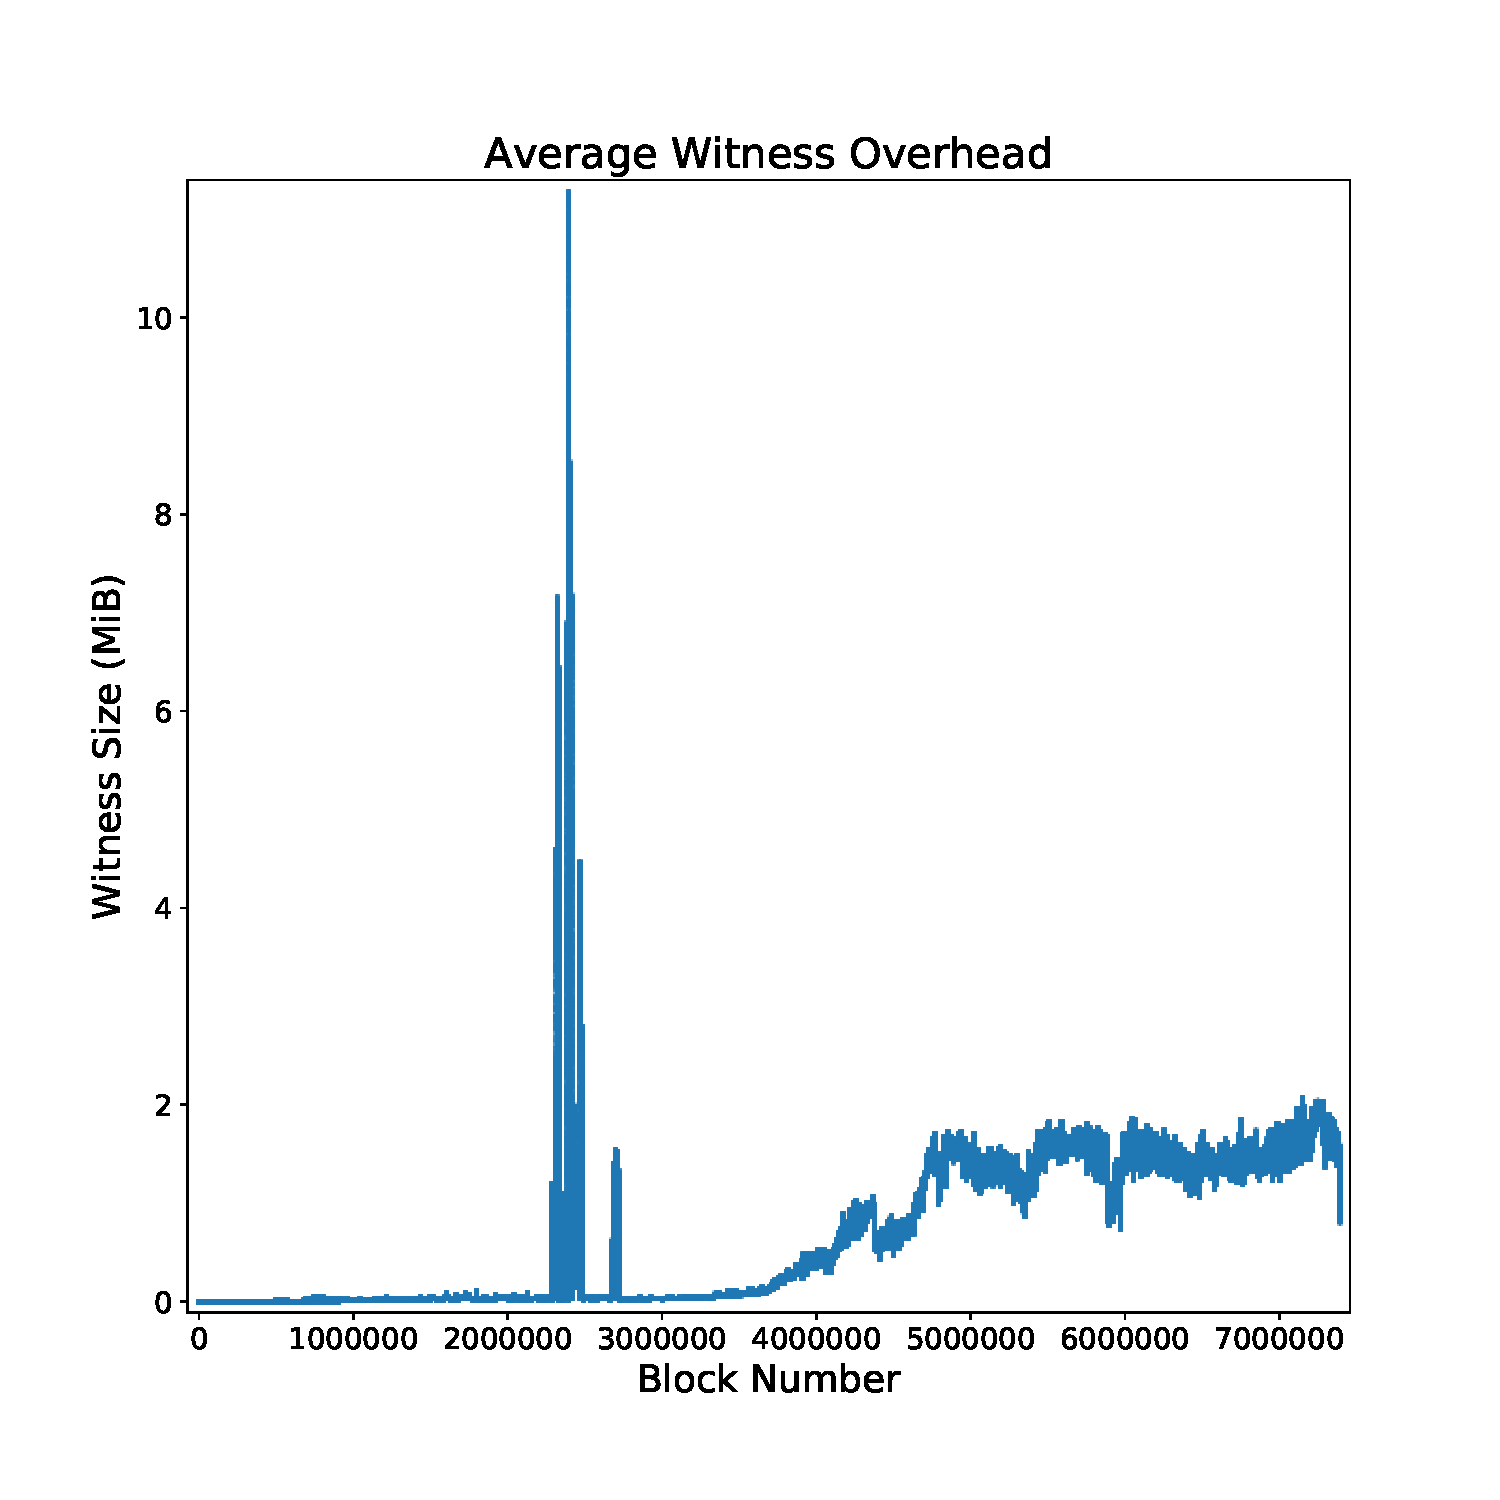
\includegraphics[width=\textwidth]{../figures/results/graphs/background/witness-size.pdf}
  \caption{Average witness size vs. block number}
  \label{fig:witnesssize}
\end{figure}

Figure~\ref{fig:witnesssize} shows the average witness size per block. There is a lot of variability in witness sizes, so the graph shows a rolling average over the last 2000 blocks at each block number. The average witness size is 723 KB over all blocks. Witness size also generally increases with block number. This is because later blocks tend to contain more transactions than earlier blocks, so more state trie nodes are required for block execution. The size of the state trie also grows as more users create Ethereum accounts, further increasing the witness size. Finally, increasing popularity of smart contracts that can potentially touch many accounts in a single transaction also contributes to witness size.

The largest witness size was 49.2 MB at block 2306350. The large spikes in the graph from blocks 2.3 to 2.7 million are from a DDoS attack on the Ethereum network in late 2016. This attack created millions of dead Ethereum accounts and significantly increased the size of the state trie. As a result, the witness sizes for blocks in this range are also very large, since they contain millions of newly created accounts.

One important detail to note is that the witness size is \emph{much} larger than the block size excluding the witness. Figure~\ref{fig:blocksize} shows the block sizes excluding the witness, which is the same as the block sizes in unmodified Ethereum.

\begin{figure}[H]
  \centering
  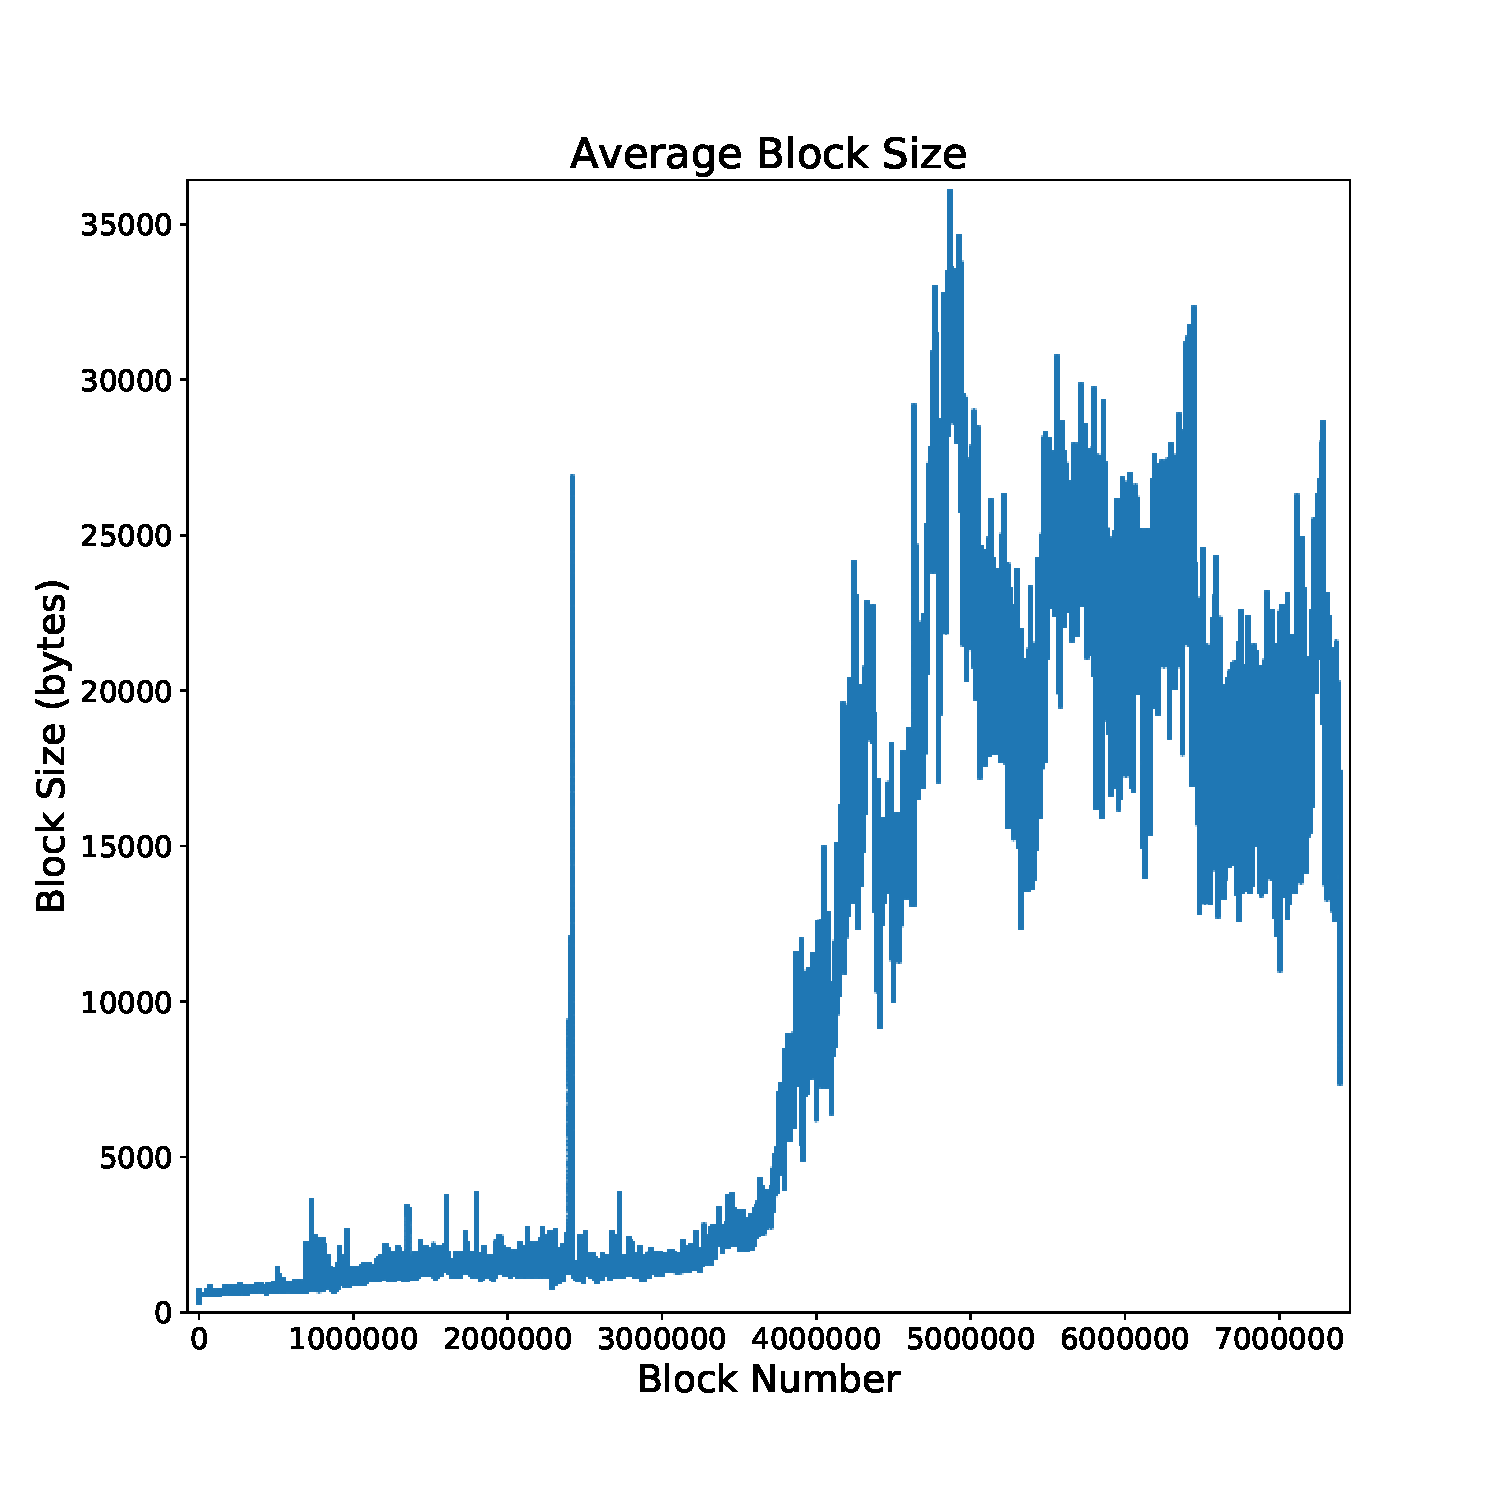
\includegraphics[width=\textwidth]{../figures/results/graphs/background/block-size.pdf}
  \caption{Average block size (excluding witness) vs. block number}
  \label{fig:blocksize}
\end{figure}


\subsubsection{Directory Size}

One closely related statistic to witness size is the directory size of the Parity data directory. Parity keeps all data inside a directory specified on the command line with the \texttt{--base-path} argument. This data includes serialized blocks and the state trie, stored in a RocksDB database. I ran a \emph{stateful} Parity node in this experiment. A stateful Parity node uses the same stateless client code, but also maintains its own state trie just as in unmodified Ethereum. Stateful nodes are useful because they act as \emph{translators}; they act as a bridge between the existing Ethereum nodes and stateless nodes by generating witnesses from existing blocks and broadcasting them on the stateless node network. The disk space required for stateful nodes is significantly larger than the space required for an unmodified Parity node, as shown in Figure~\ref{fig:ondisksize}.

\begin{figure}[H]
  \centering
  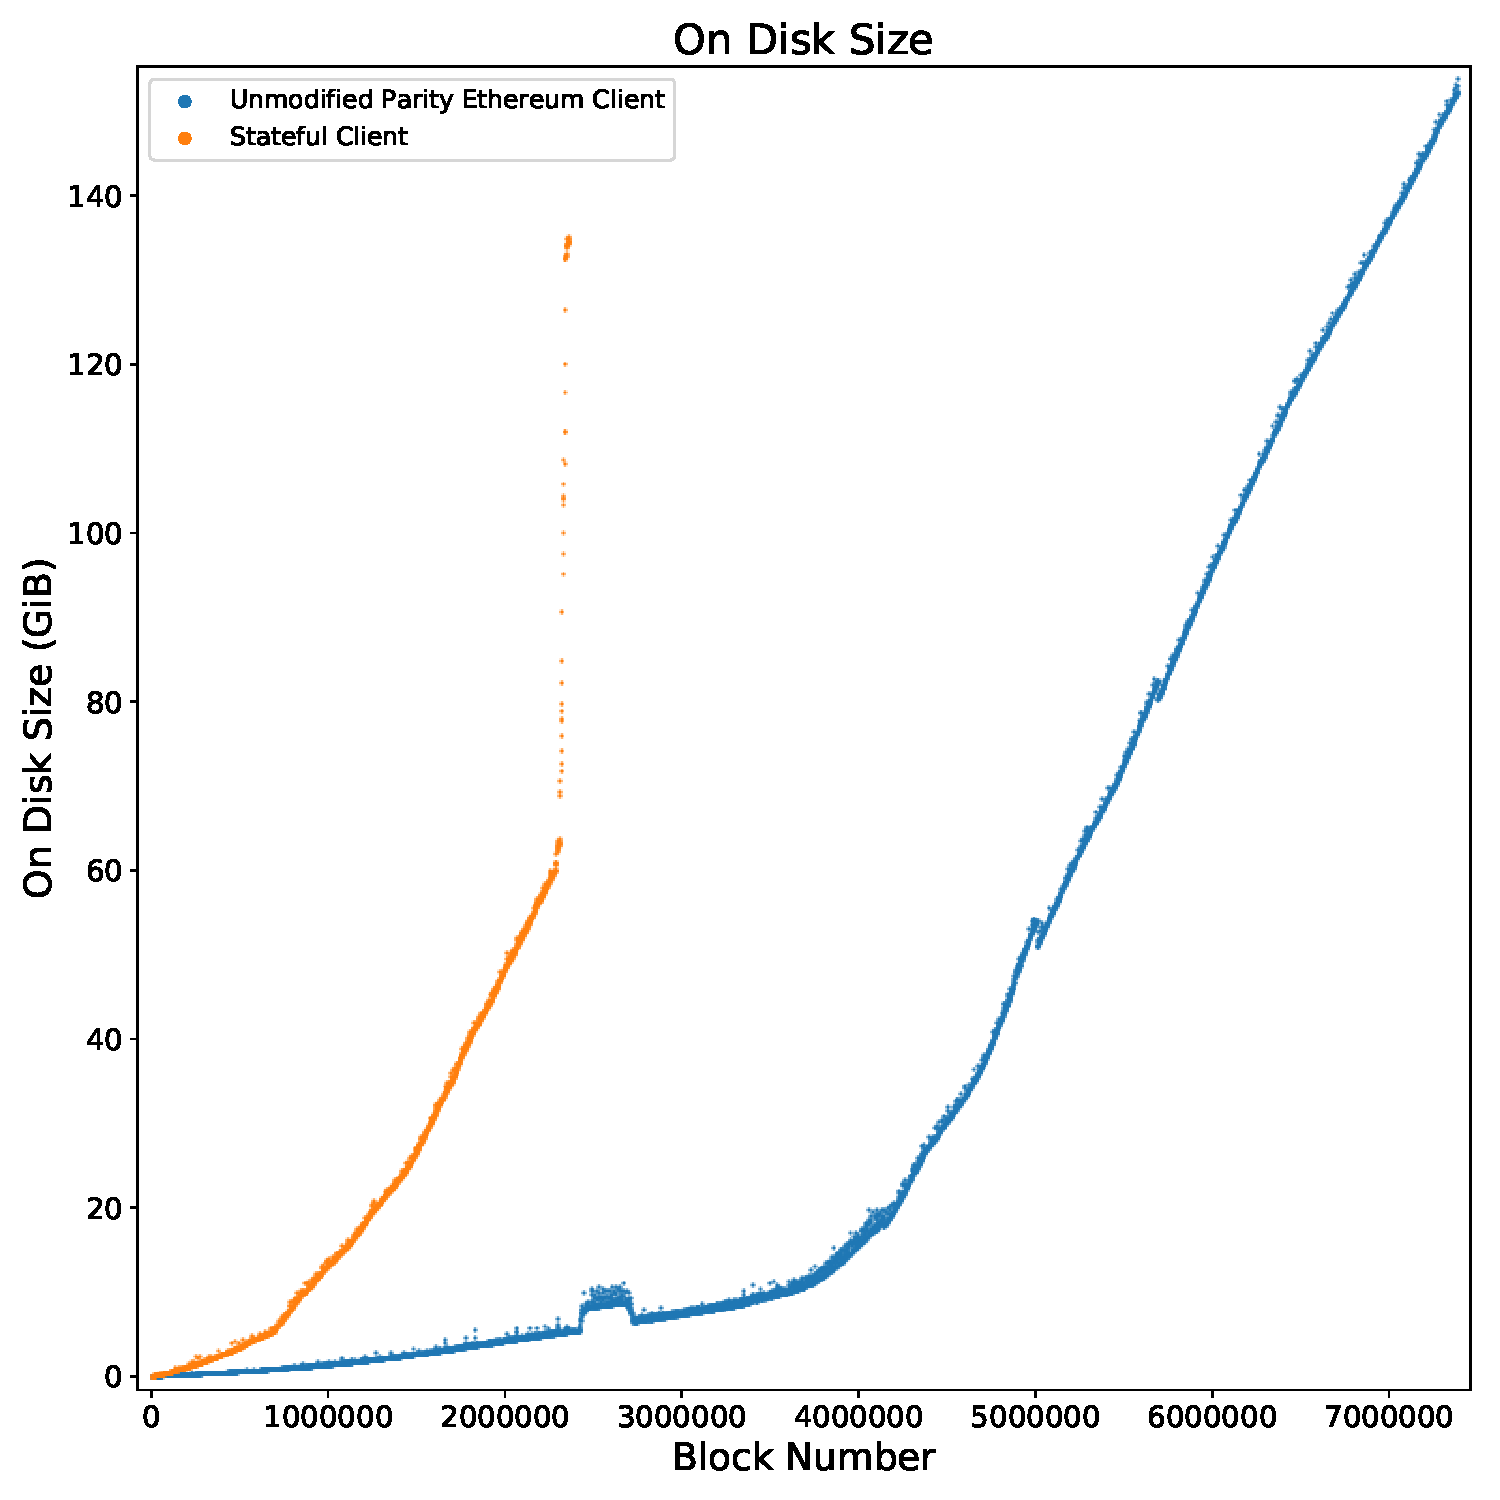
\includegraphics[width=\textwidth]{../figures/results/graphs/background/on-disk-size.pdf}
  \caption{On disk size of stateful client and unmodified client, per block number.}
  \label{fig:ondisksize}
\end{figure}

The disk space required for running a stateful client grows much more quickly than for running an unmodified Parity client. Due to space constraints, stateful client disk usage was only able to be collected for the first 2.3 million blocks. However, using the data from Figures~\ref{fig:witnesssize}~and~\ref{fig:blocksize}, we are able to project what the on disk size would be if the experiment had continued.

\begin{figure}[H]
  \centering
  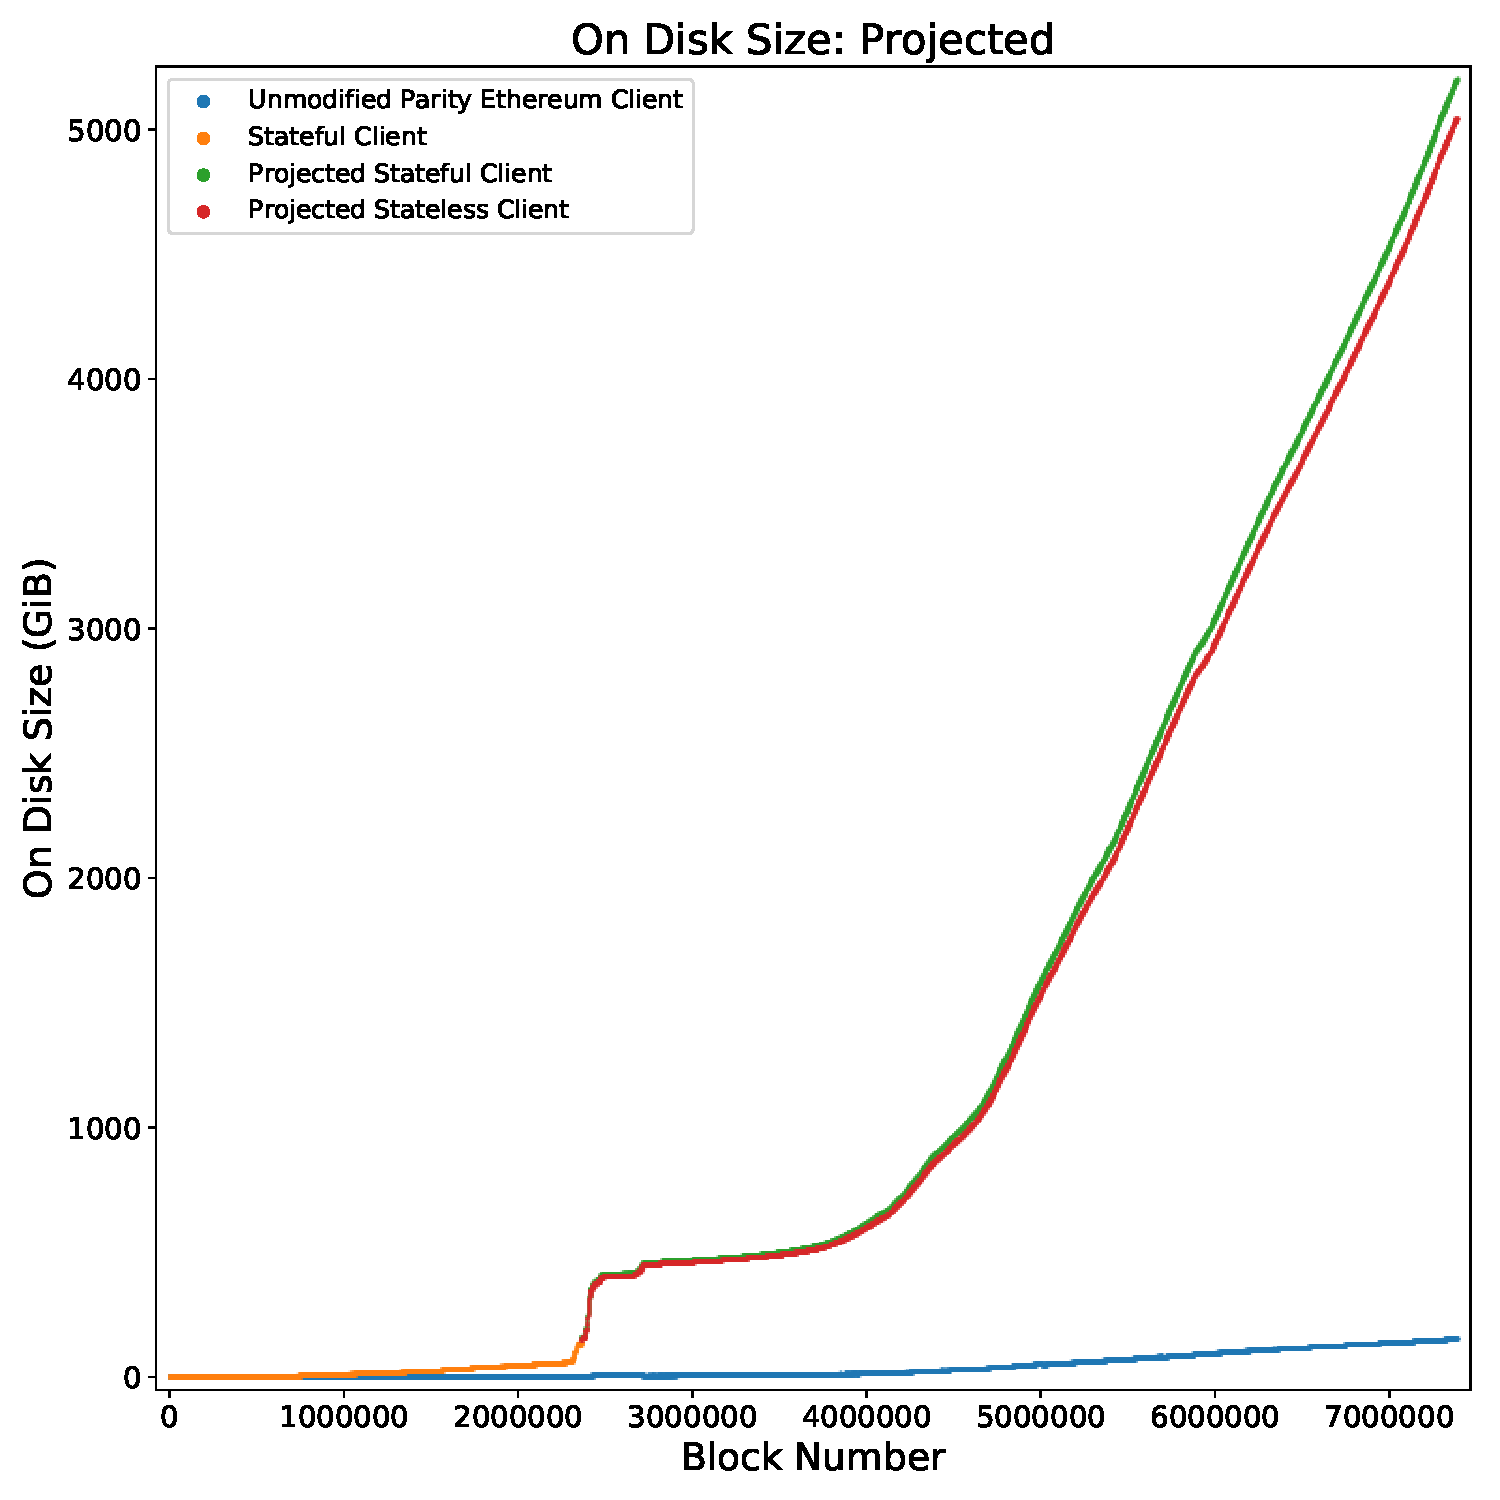
\includegraphics[width=\textwidth]{../figures/results/graphs/background/projected-on-disk-size.pdf}
  \caption{Projected on disk size of stateful client and stateless client, compared to actual on disk size of unmodified client.}
  \label{fig:projectedondisksize}
\end{figure}

The projected data in Figure~\ref{fig:projectedondisksize} was obtained by using cumulative sums of block size and witness size. If this experiment had continued, then the actual disk usage would be slightly less than the proejcted usage. This is because RocksDB compresses blockchain data. However, even with the projected data it is apparent that the space required to store witnesses for each block makes the stateless clients proposal impractical. Currently a new Ethereum block is mined every 15 seconds. Using the projected rate of disk usage growth, 1.7 MB of data will have to be stored per new block, amounting to 9.8 GB of additional disk usage per day.

\subsubsection{Verification Time}

\subsubsection{Database Operations}

One advantage of stateless clients is that the number of database operations is greatly reduced. Compare the amount of operations done in unmodified Ethereum INSERT FIGURE HERE (ALREADY HAVE DATA). The number of database operations for stateless clients is constant (IS THIS TRUE? NEED TO CHECK)

\section{Related Work}

There are several other potential solutions to scaling blockchains.

\subsection{Ethereum 2.0 Sharding}

Stateless clients is part of a larger effort within the Ethereum community to develop \emph{Ethereum 2.0}. Ethereum 2.0 is a set of specifications for the next version of Ethereum. One of the ideas proposed in Ethereum 2.0 is to \emph{shard} the blockchain. Currently, all Ethereum nodes process all transactions. Once a block is mined, it is broadcast to the whole network and every Ethereum node verifies the block independently. The problem with this approach is that the throughput of the entire system is limited by the throughput of a single node.

Ethereum 2.0 Sharding proposes to split the blockchain and state trie into partitions called \emph{``shards''}. One sharding scheme is to create shards based on account addresses. For example, all account addresses starting with \texttt{0x0...} would be in one shard, all account addresses starting with \texttt{0x1...} would be in another shard, and so on until account addresses starting with \texttt{0xf...}. This scheme creates 16 shards, one for each hexadecimal digit from \texttt{0x0} to \texttt{0xf}. Within a shard, Ethereum transactions are the same as in the current version of Ethereum. Intra-shard transaction execution is not changed, but there is a complex protocol to handle inter-shard transactions. % TODO: explain this?

\subsection{Hyperledger Fabric}



\subsection{RainBlock} \label{subsection:rainblock}



\section{Future Work}

One area that could be explored in the future is different techniques for reducing witness size. In Section~\ref{subsection:results}, I showed how the witness sizes make the stateless clients proposal impractical to use. However, using techniques such as witness revision and caching, it is possible that witness sizes could be reduced. RainBlock (Section~\ref{subsection:rainblock}) does this.


\section{Conclusion}

\end{document}
